Rancangan arsitektur sistem dapat dilihat pada Gambar \ref{fig:arsitektur-sistem}. Sistem ini terdiri dari 3 komponen utama yaitu komponen \textit{data preprocessing}, komponen \textit{data mining}, dan komponen \textit{data integration}. Komponen \textit{data preprocessing} berfungsi untuk membersihkan data dari \textit{noise} dan \textit{outlier}. Komponen \textit{data mining} berfungsi untuk melakukan analisis risiko autentikasi dengan menggunakan metode Random Forest. Komponen \textit{data integration} berfungsi untuk mengintegrasikan sistem dengan sistem FHIR.

\begin{figure}[H]
    \centering
    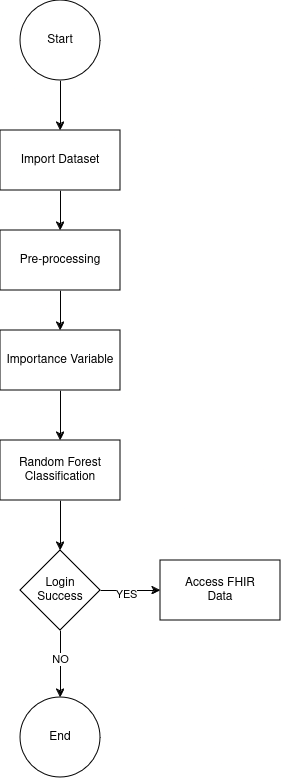
\includegraphics[width=0.5\textwidth]{BAB_TESIS/IMAGES/diagram_kusus.drawio.png}
    \caption{Rancangan Arsitektur Sistem}
    \label{fig:arsitektur-sistem}
\end{figure}

Pada Gambar \ref{fig:arsitektur-sistem}, sistem ini akan mendapatkan data login dari datasest. Data login ini kemudian akan digunakan sebagai input untuk melakukan analisis risiko autentikasi. Dalam menentukan risiko autentikasi, sistem ini akan menggunakan metode Random Forest. Metode Random Forest akan menghasilkan variabel kepentingan yang dapat digunakan untuk melakukan analisis risiko autentikasi.

Setelah itu, sistem ini akan terintegrasi dengan sistem FHIR. Sistem ini akan menggunakan FHIR API untuk mengakses data dari sistem FHIR. FHIR API akan mengakses data dari sistem FHIR dengan menggunakan \textit{request} dan \textit{response}.